\chapter{Testing and Evaluation}

\section{Testing}

To test PyPltRedex, two forms of testing are employed: 

\begin{enumerate}
\item Unit testing form most non-trivial transformation / analysis passes.
\item Integration tests containing \texttt{redex-match-assert-equal}, \texttt{term-let-assert-equal}, \texttt{apply-reduction-relation-assert-equal} forms that test functionality of pattern matching, term-generation and application of reduction relations and metafunctions. Some tests cases were lifted from a testing suite that comes with PLTRedex. All test cases use the output of PLTRedex for comparison.
\end{enumerate}

\section{Performance}

To get a feel for how PyPyPLTRedex would stack up against PLTRedex in terms performance, the Imp language was used to implement a simple iterative factorial calculator seen in Figure \ref{imp-factorial}. The program correctly computed factorial of 20 producing 2432902008176640000; factorial was evaluated 1000 times to obtain more reliable data. The program was also implemented in plain Python and compiled with the RPython toolchain. All programs were run three times and the resulting times were averaged. Results of profiling can be seen in Figure \ref{perf-fact}.

\begin{figure}[h]
\begin{minted}[tabsize=2,obeytabs,escapeinside=//,mathescape=true,fontsize=\normalsize]{python}
{
	(N = 20)
	(product = 1)
	(i = 1)
	[while (i <= N)
		(product = (product * i))
		(i = (i + 1))]
}
\end{minted}
\caption{Factorial program implemented in Imp.}
\label{imp-factorial}
\end{figure}

Benchmarking is set up in the way seen in Figure \ref{bench-setup}. Actual running time is measured with the utility \texttt{perf} and \texttt{chrt} is used to minimize context switches.

\begin{figure}[h]
\begin{minted}[tabsize=2,obeytabs,fontsize=\normalsize]{text}
sudo chrt -f 99 perf stat ./benc_fact/fact-c 
\end{minted}
\caption{Benchmarking setup.}
\label{bench-setup}
\end{figure}


\begin{figure}[h]
\centering
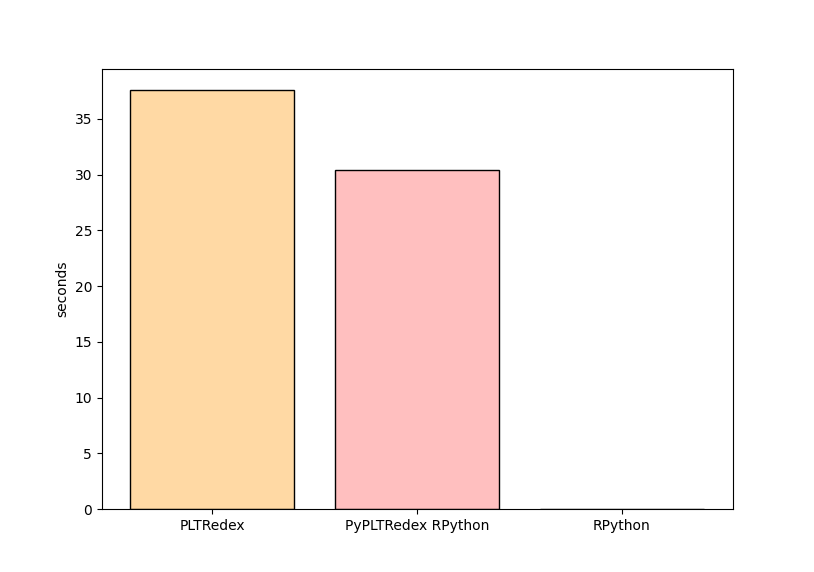
\includegraphics[scale=0.7]{perf-fact.png}
\caption{Profiling \texttt{Factorial(20)} program.}
\label{perf-fact}
\end{figure}
